% BEGIN LICENSE BLOCK
% Version: CMPL 1.1
%
% The contents of this file are subject to the Cisco-style Mozilla Public
% License Version 1.1 (the "License"); you may not use this file except
% in compliance with the License.  You may obtain a copy of the License
% at www.eclipse-clp.org/license.
% 
% Software distributed under the License is distributed on an "AS IS"
% basis, WITHOUT WARRANTY OF ANY KIND, either express or implied.  See
% the License for the specific language governing rights and limitations
% under the License. 
% 
% The Original Code is  The ECLiPSe Constraint Logic Programming System. 
% The Initial Developer of the Original Code is  Cisco Systems, Inc. 
% Portions created by the Initial Developer are
% Copyright (C) 2006 Cisco Systems, Inc.  All Rights Reserved.
% 
% Contributor(s): 
% 
% END LICENSE BLOCK

\chapter{Tree Search Methods}
\label{chapsearch}
%HEVEA\cutdef[1]{section}
%----------------------------------------------------------------------
\section{Introduction}
%----------------------------------------------------------------------
In this chapter we will take a closer look at the principles and
\index{alternative search methods}
alternative methods of searching for solutions in the presence of
constraints. Let us first recall what we are talking about.
We assume we have the standard pattern of a constraint program:
\begin{code}
solve(Data) :-
        model(Data, Variables),
        search(Variables),
        print_solution(Variables).
\end{code}
The model part contains the logical {\em model} of our problem. It defines
the variables and the constraints.
Every variable has a {\em domain} of values that it can take
(in this context, we only consider domains with a finite number of values).

Once the model is set up, we go into the search phase.
Search is necessary since generally the implementation of the constraints
is not complete, i.e.\ not strong enough to logically infer directly
the solution to the problem. Also, there may be multiple solutions
which have to be located by search, e.g.\ in order to find the best one.
In the following, we will use the following terminology:
\begin{itemize}
\item If a variable is given a value (from its domain, of course),
    \index{assignment}
        we call this an {\em assignment}. If every problem variable is given
        a value, we call this a {\em total assignment}.
\item A total assignment is a {\em solution} if it satisfies all the
        constraints.
\item The {\em search space} is the set of all possible total assignments.
    \index{search space}
        The search space is usually very large because it grows exponentially
        with the problem size:
        \begin{displaymath}
        SearchSpaceSize = {DomainSize}^{NumberOfVariables}
        \end{displaymath}
\end{itemize}


% - - - - - - - - - - - - - - - - - - - - - - - - - - - - - - - - - - -
\subsection{Overview of Search Methods}
% - - - - - - - - - - - - - - - - - - - - - - - - - - - - - - - - - - -

\begin{figure}
\begin{center}
\resizebox{0.55\textwidth}{!}{
\includegraphics{search3.eps}}
\end{center}
\caption{A search space of size 16}
\label{figsearchspace}
\end{figure}
Figure \ref{figsearchspace} shows a search space with N (here 16)
possible total assignments, some of which are solutions.
Search methods now differ in the way in which these assignments
are visited.
We can classify search methods according to different criteria:
\begin{description}
\item[Complete vs incomplete exploration] complete search means that the search space
    \index{complete search}
    \index{incomplete search}
    is investigated in such a way that all solutions are guaranteed to be found.
    This is necessary when the optimal solution is needed (one has to prove
    that no better solution exists). Incomplete search may be sufficient when
    just some solution or a relatively good solution is needed.
\item[Constructive vs move-based] this indicates whether the method advances
    \index{constructive search}
    \index{move-based search}
    by incrementally constructing assignments (thereby reasoning about partial
    assignments which represent subsets of the search space) or by moving
    between total assignments (usually by modifying previously explored
    assignments).
\item[Randomness] some methods have a random element while others follow
    \index{random search}
    fixed rules.
\end{description}
Here is a selection of search methods together with their properties:

\begin{center}
\begin{tabular}{|l|lll|}
\hline
Method&                 exploration&    assignments&    random\\
\hline
Full tree search&       complete&       constructive&   no\\
Credit search&          incomplete&     constructive&   no\\
Bounded backtrack&      incomplete&     constructive&   no\\
Limited discrepancy&    complete&       constructive&   no\\
Hill climbing&          incomplete&     move-based&     possibly\\
Simulated annealing&    incomplete&     move-based&     yes\\
Tabu search&            incomplete&     move-based&     possibly\\
Weak commitment&        complete&       hybrid&         no\\
\hline
\end{tabular}
\end{center}

\index{tree search}
\index{search tree}
The constructive search methods usually organise the search space by
partitioning it systematically.  This can be done naturally with a
search tree (Figure \ref{figsearchtree}).  The nodes in this tree
represent choices which partition the remaining search space into two
or more (usually disjoint) sub-spaces.  Using such
a tree structure, the search space can be traversed systematically and
completely (with as little as O(N) memory requirements).

\begin{figure}
\begin{center}
\resizebox{0.55\textwidth}{!}{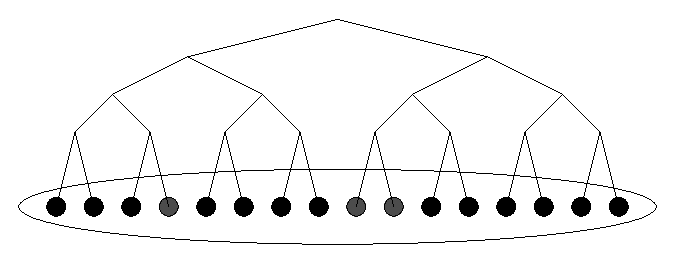
\includegraphics{search4.eps}}
\end{center}
\caption{Search space structured using a search tree}
\label{figsearchtree}
\end{figure}
Figure \ref{figtreesearch} shows a sample tree search, namely a depth-first
incomplete traversal.
As opposed to that, figure \ref{figmovesearch} shows an example of an
incomplete move-based search which does not follow a fixed search space
structure. Of course, it will have to take other precautions to avoid
looping and ensure termination.
\begin{figure}
\begin{center}
\resizebox{0.55\textwidth}{!}{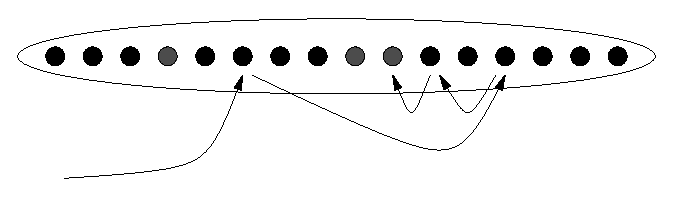
\includegraphics{search5.eps}}
\end{center}
\caption{A move-based search}
\label{figmovesearch}
\end{figure}

\begin{figure}
\begin{center}
\resizebox{0.55\textwidth}{!}{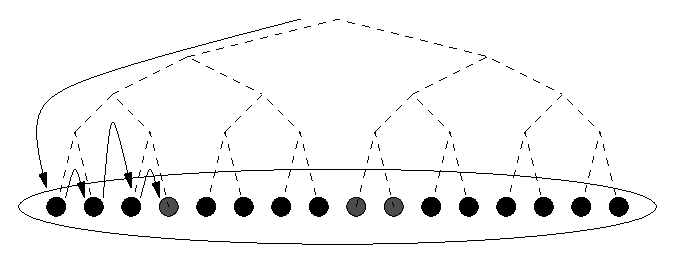
\includegraphics{search6.eps}}
\end{center}
\caption{A tree search (depth-first)}
\label{figtreesearch}
\end{figure}

A few further observations:
Move-based methods are usually incomplete. This is not surprising given
typical sizes of search spaces.
A complete exploration of a huge search space
is only possible if large sub-spaces can be excluded a priori, and this
is only possible with constructive methods which allow one to reason about
whole classes of similar assignments.
Moreover, a complete search method must remember which parts of the
search space have already been visited.
This can only be implemented with
acceptable memory requirements if there is a simple structuring of the
space that allows compact encoding of sub-spaces.


% - - - - - - - - - - - - - - - - - - - - - - - - - - - - - - - - - - -
\subsection{Optimisation and Search}
% - - - - - - - - - - - - - - - - - - - - - - - - - - - - - - - - - - -
\label{secbboptsearch}
\index{optimisation}
Many practical problems are in fact optimisation problems, ie.\ we are
not just interested in some solution or all solutions, but in
the best solution.

Fortunately, there is a general method to find the optimal solution
based on the ability to find all solutions.
\index{branch-and-bound}
The {\em branch-and-bound} technique works as follows:
\begin{enumerate}
\item Find a first solution
\item Add a constraint requiring a better solution than the best
    one we have so far (e.g.\ require lower cost)
\item Find a solution which satisfies this new constraint.
    If one exists, we have a new best solution and we repeat step 2.
    If not, the last solution found is the proven optimum.
\end{enumerate}
The {\em branch\_and\_bound} library provides generic predicates 
which implement this technique:
\begin{description}
\item[minimize(+Goal,-Cost)]
This is the simplest predicate in the {\em branch_and_bound} library:
A solution of the goal {\it Goal} is found that minimizes the value of
{\em Cost}. {\em Cost} should be a variable that is affected, and 
eventually instantiated, by the execution of {\it Goal}. Usually, {\it Goal}
is the search procedure of a constraint problem and {\it Cost} is the variable
representing the cost.

\item[bb_min(+Goal, -Cost, ++Options)]
A more flexible version where the programmer can take more control
over the branch and bound behaviour and choose between different
strategies and parameter settings.
\end{description}


% - - - - - - - - - - - - - - - - - - - - - - - - - - - - - - - - - - -
\subsection{Heuristics}
% - - - - - - - - - - - - - - - - - - - - - - - - - - - - - - - - - - -

Since search space sizes grow exponentially with problem size,
it is not possible to explore all assignments except for the
very smallest problems.
The only way out is {\em not} to look at the whole search space.
There are only two ways to do this:
\begin{itemize}
\item {\bf Prove} that certain areas of the space contain no solutions.
    This can be done with the help of constraints. This is often referred
    to as {\em pruning}\index{pruning}.
\item {\bf Ignore} parts of the search space that are unlikely to contain
    solutions (i.e.\ do incomplete search), or at least postpone their exploration.
    This is done by using {\em heuristics}\index{heuristics}.
    A heuristic is a particular traversal order of the search space
    which explores promising areas first.
\end{itemize}

In the following sections we will first investigate the considerable
degrees of freedom that are available for heuristics within the framework of
systematic tree search, which is the traditional search method
in the Constraint Logic Programming world.

Subsequently, we will turn our attention to move-based methods
which in {\eclipse} can be implemented using the facilities of the 
{\tt repair} library.


%----------------------------------------------------------------------
\section{Complete Tree Search with Heuristics}
%----------------------------------------------------------------------

\index{complete search}
There is one form of tree search which is especially economic: 
depth-first, left-to-right search by backtracking.  It allows
a search tree to be traversed systematically while requiring only a stack
of maximum depth N for bookkeeping.  Most other strategies of tree
search (e.g.  breadth-first) have exponential memory requirements. 
This unique property is the reason why backtracking is a built feature
of {\eclipse}.  Note that the main disadvantage of the depth-first
strategy (the danger of going down an infinite branch) does not come
into play here because we deal with finite search trees.

\index{depth-first search}
Sometimes depth-first search and heuristic search are treated as antonyms.
This is only justified when the shape of the search tree is statically fixed.
Our case is different: we have the freedom of deciding on the shape of every
sub-tree before we start to traverse it depth-first. While this does not
allow for absolutely {\em any} order of visiting the leaves of the search tree,
it does provide considerable flexibility. This flexibility can be exploited
by variable and value selection strategies.

% - - - - - - - - - - - - - - - - - - - - - - - - - - - - - - - - - - -
\subsection{Search Trees}
% - - - - - - - - - - - - - - - - - - - - - - - - - - - - - - - - - - -

In general, the nodes of a search tree represent {\em choices}.
\index{choice}
These choices should be mutually exclusive and therefore partition the
\index{partition a search space}
search space into two or more disjoint sub-spaces.
In other words, the original problem is reduced to a disjunction
of simpler sub-problems.

In the case of finite-domain problems, the most common form of choice
is to choose a particular value for a problem variable
(this technique is often called
\index{labeling}
{\em labeling}).
For a boolean variable, this means setting the variable to 0 in one
branch of the search tree and to 1 in the other.
In {\eclipse}, this can be written as a disjunction
(which is implemented by backtracking):
\begin{quote}\begin{alltt}
( X1=0 ; X1=1 )
\end{alltt}\end{quote}
Other forms of choices are possible. If X2 is a variable that can take
integer values from 0 to 3 (assume it has been declared as \verb'X2::0..3'),
we can make a n-ary search tree node by writing
\begin{quote}\begin{alltt}
( X2=0 ; X2=1 ; X2=2 ; X2=3 )
\end{alltt}\end{quote}
or more compactly
\begin{quote}\begin{alltt}
indomain(X2)
\end{alltt}\end{quote}
However, choices do not necessarily involve choosing a concrete value
for a variable. It is also possible to make disjoint choices by
\index{domain splitting}
{\em domain splitting}, e.g.
\begin{quote}\begin{alltt}
( X2 #=< 1 ; X2 #>= 2 )
\end{alltt}\end{quote}
or by choosing a value in one branch and excluding it in the other:
\begin{quote}\begin{alltt}
( X2 = 0 ; X2 #>= 1 )
\end{alltt}\end{quote}
In the following examples, we will mainly use simple labeling,
which means that the search tree nodes correspond to a variable
and a node's branches correspond to the different values that the
variable can take.


% - - - - - - - - - - - - - - - - - - - - - - - - - - - - - - - - - - -
\subsection{Variable Selection}
\index{variable selection}
% - - - - - - - - - - - - - - - - - - - - - - - - - - - - - - - - - - -

\begin{figure}
\begin{center}
\resizebox{0.5\textwidth}{!}{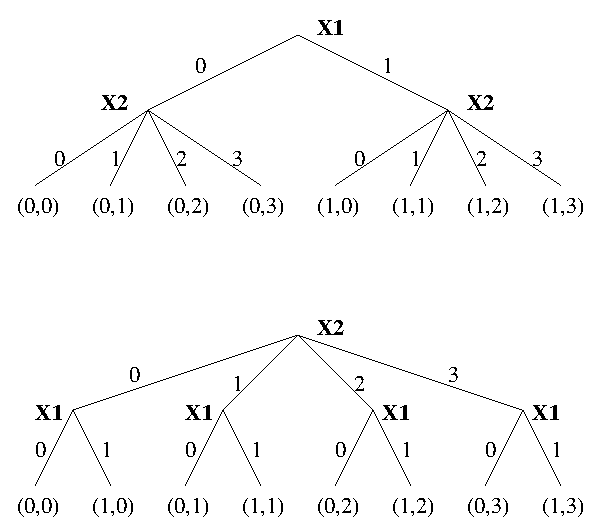
\includegraphics{search1.eps}}
\end{center}
\caption{The effect of variable selection}
\label{figvarsel}
\end{figure}

Figure \ref{figvarsel} shows how variable selection reshapes a search tree.
If we decide to choose values for X1 first (at the root of the search tree)
and values for X2 second, then the search tree has one particular shape.
If we now assume a depth-first, left-to-right traversal by backtracking,
this corresponds to one particular order of visiting the leaves of the tree:
(0,0), (0,1), (0,2), (0,3), (1,0), (1,1), (1,2), (1,3).

If we decide to choose values for X2 first and X1 second, then the tree and
consequently the order of visiting the leaves is different:
(0,0), (1,0), (0,1), (1,1), (0,2), (1,2), (0,3), (1,3).

While with 2 variables there are only 2 variable selection strategies,
this number grows exponentially with the number of variables. For 5
variables there are already $2^{2^{5}-1} = 2147483648$ different variable selection
strategies to choose from.

Note that the example shows something else: If the domains of the variables
are different, then the variable selection can change the number of internal
nodes in the tree (but not the number of leaves). To keep the number of nodes
down, variables with small domains should be selected first.


% - - - - - - - - - - - - - - - - - - - - - - - - - - - - - - - - - - -
\subsection{Value Selection}
\index{value selection}
% - - - - - - - - - - - - - - - - - - - - - - - - - - - - - - - - - - -

The other way to change the search tree is value selection, i.e. reordering
the child nodes of a node by choosing the 
values from the domain of a variable in a particular order.
Figure \ref{figvalsel} shows how this can change the order of visiting the
leaves:
(1,2), (1,1), (1,0), (1,3), (0,1), (0,3), (0,0), (0,2).

\begin{figure}
\begin{center}
\resizebox{0.5\textwidth}{!}{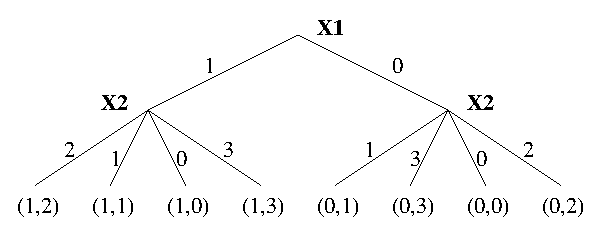
\includegraphics{search2.eps}}
\end{center}
\caption{The effect of value selection}
\label{figvalsel}
\end{figure}

By combining variable and value selection alone, a large number of different
heuristics can be implemented.
To give an idea of the numbers involved, table \ref{visits} shows the search
space sizes, the number of possible search space traversal orderings,
and the number of orderings
that can be obtained by variable and value selection (assuming domain size 2).

\begin{figure}[t]
\enableunderscores
\begin{center}
\begin{tabular}{|l|l|l|l|}
\hline
Variables&      Search space&   Visiting orders&        Selection Strategies\\
\hline
1&              2&                      2&              2\\
2&              4&                      24&             16\\
3&              8&                      40320&          336\\
4&              16&                     $2.1*10^{13}$&  $1.8*10^7$\\
5&              32&                     $2.6*10^{35}$&  $3.5*10^{15}$\\
n&              $2^n$&          $2^n!$& 
                                $2^{{2^n}-1} \prod_{i=0}^{n-1} (n-1)^{2^i}$\\
\hline
\end{tabular}
\end{center}
\caption{Flexibility of Variable/Value Selection Strategies}
\label{visits}
\disableunderscores
\end{figure}

% - - - - - - - - - - - - - - - - - - - - - - - - - - - - - - - - - - -
\subsection{Example}
% - - - - - - - - - - - - - - - - - - - - - - - - - - - - - - - - - - -

\index{queens}
We use the famous N-Queens problem to illustrate how heuristics can be applied
to backtrack search through variable and value selection.
We model the problem with one variable per queen, assuming that each queen
occupies one colunm. The variables range from 1 to N and indicate the row
in which the queen is being placed. The constraints ensure that no two
queens occupy the same row or diagonal:
\label{queenscode}
\begin{code}
:- lib(ic).

queens(N, Board) :-
        length(Board, N),
        Board :: 1..N,
        ( fromto(Board, [Q1|Cols], Cols, []) do
            ( foreach(Q2, Cols), count(Dist,1,_), param(Q1) do
                noattack(Q1, Q2, Dist)
            )
        ).

    noattack(Q1,Q2,Dist) :-
        Q2 #\verb.\.= Q1,
        Q2 - Q1 #\verb.\.= Dist,
        Q1 - Q2 #\verb.\.= Dist.
\end{code}
We are looking for a first solution to the 16-queens problem by calling
\begin{quote}\begin{alltt}
?- queens(16, Vars),   % model
   labeling(Vars).     % search
\end{alltt}\end{quote}
We start naively, using the pre-defined labeling-predicate that comes with the
{\em ic} library. It is defined as follows:
\begin{code}
labeling(AllVars) :-
        ( foreach(Var, AllVars) do
            indomain(Var)                       % select value
        ).
\end{code}
The strategy here is simply to select the variables
from left to right as they occur in the list, and they are
assigned values starting from the lowest to the numerically highest they can
take (this is the definition of indomain/1).
A solution is found after 542 backtracks
(see section \ref{countbt} below for how to count backtracks).

A first improvement is to employ a
{\bf general-purpose variable-selection heuristic},
\index{first-fail principle}
the so called first-fail principle. It requires to label the
variables with the smallest domain first. This reduces the branching
factor at the root of the search tree and the total number of internal nodes.
\index{ic_search}
The delete/5 predicate from the {\em ic_search} library
implements this strategy for finite integer domains.
Using delete/5, we can redefine our labeling-routine as follows:
\begin{code}
:- lib(ic_search).
labeling_b(AllVars) :-
        ( fromto(AllVars, Vars, VarsRem, []) do
            delete(Var, Vars, VarsRem, 0, first_fail), % dynamic var-select
            indomain(Var)                              % select value
        ).
\end{code}
Indeed, for the 16-queens example, this leads to a dramatic improvement,
the first solution is found with only 3 backtracks now.
But caution is necessary: The 256-queens instance for example solves
nicely with the naive strategy, but our improvement leads to a
disappointment: the time increases dramatically!
This is not uncommmon with heuristics: one has to keep in mind that the
search space is not reduced, just re-shaped. Heuristics that yield good
results with some problems can be useless or counter-productive with others.
Even different instances of the same problem can exhibit widely different
characteristics.
 
Let us try to employ a {\bf problem-specific heuristic}:
\index{problem-specific heuristic}
Chess players know that pieces in the middle of the board are more
useful because they can attack more fields. We could therefore start
placing queens in the middle of the board to reduce the number of
unattacked fields earlier. We can achieve that simply by pre-ordering the
variables such that the middle ones are first in the list:
\begin{code}
labeling_c(AllVars) :-
        middle_first(AllVars, AllVarsPreOrdered), % static var-select
        ( foreach(Var, AllVarsPreOrdered) do
            indomain(Var)                         % select value
        ).
\end{code}
The implementation of middle\_first/2 requries a bit of list manipulation
\index{middle-first}
and uses primitives from the lists-library:
\begin{code}
:- lib(lists).

middle_first(List, Ordered) :-
        halve(List, Front, Back),
        reverse(Front, RevFront),
        splice(Back, RevFront, Ordered).
\end{code}
This strategy also improves things for the 16-queens instance, the
first solution requires 17 backtracks.

We can now improve things further by {\bf combining} the two
variable-selection strategies:
When we pre-order the variables such that the middle ones are first,
\index{delete/5}
the delete/5 predicate will prefer middle variables when several
have the same domain size:
\begin{code}
labeling_d(AllVars) :-
        middle_first(AllVars, AllVarsPreOrdered), % static var-select
        ( fromto(AllVarsPreOrdered, Vars, VarsRem, []) do
            delete(Var, Vars, VarsRem, 0, first_fail),  % dynamic var-select
            indomain(Var)                       % select value
        ).
\end{code}
The result is positive: for the 16-queens instance,
the number of backtracks goes down to zero,
and more difficult instances become solvable!

Actually, we have not yet implemented our intuitive heuristics properly.
We start placing queens in the middle columns, but not on the middle rows.
With our model, that can only be achieved by {\bf changing the value selection},
ie.\ setting the variables to values in the middle of their domain first.
For this we can use indomain/2, a more flexible variant of indomain/1,
provided by the {\em ic_search} library.
It allows us to specify that we want to start labeling with the middle value
in the domain:
\begin{code}
labeling_e(AllVars) :-
        middle_first(AllVars, AllVarsPreOrdered), % static var-select
        ( fromto(AllVarsPreOrdered, Vars, VarsRem, []) do
            delete(Var, Vars, VarsRem, 0, first_fail),  % dynamic var-select
            indomain(Var, middle)                 % select value
        ).
\end{code}
Surprisingly, this improvement again increases the backtrack count for
16-queens again to 3.
However, when looking at a number of different instances of the problem,
we can observe that the overall behaviour has improved and the
performance has become more predictable than with the
initial more naive strategies.
Figure \ref{queensresult} shows the behaviour of the different
strategies on various problem sizes.
\begin{figure}
\begin{center}
\begin{tabular}{l|l|l|l|l|l|l|l|l}
N =     &8  &12 &14 &16 &32 &64 &128    &256\\
\hline
labeling_a  &10 &15 &103    &542    &   &   &   &\\
labeling_b  &10 &16 &11 &3  &4  &148    &   &\\
labeling_c  &0  &3  &22 &17 &   &   &   &\\
labeling_d  &0  &0  &1  &0  &1  &1  &   &\\
labeling_e  &3  &3  &38 &3  &7  &1  &0  &0\\
\end{tabular}
\end{center}
\label{queensresult}
\caption{N-Queens with different labeling strategies: Number of backtracks}
\end{figure}



% - - - - - - - - - - - - - - - - - - - - - - - - - - - - - - - - - - -
\subsection{Counting Backtracks}
\index{backtrack count}
% - - - - - - - - - - - - - - - - - - - - - - - - - - - - - - - - - - -

%The size of the (remaining) search space can be computed easily
%in finite-domain problems. All we have to do is to multiply the
%sizes of all the (remaining) variable's domains:
%\begin{quote}\begin{alltt}
%search_space(Vars, Size) :-
%        ( foreach(V,Vars), fromto(1,S0,S1,Size) do
%            dvar_domain(V,D), S1 is S0*dom_size(D)
%        ).
%\end{alltt}\end{quote}

\label{countbt}
An interesting piece of information during program development is the
number of backtracks. It is a good measure for the quality of
both constraint propagation and search heuristics.
We can instrument our labeling routine as follows:
\begin{code}
labeling(AllVars) :-
        init_backtracks,
        ( foreach(Var, AllVars) do
            count_backtracks,       % insert this before choice!
            indomain(Var)
        ),
        get_backtracks(B),
        printf("Solution found after %d backtracks%n", [B]).
\end{code}
The backtrack counter itself can be implemented by the code below.
It uses a non-logical counter variable (backtracks) and an additional
flag (deep\_fail) which ensures that backtracking to exhausted choices
does not increment the count.
\begin{code}
:- local variable(backtracks), variable(deep_fail).

init_backtracks :-
        setval(backtracks,0).

get_backtracks(B) :-
        getval(backtracks,B).

count_backtracks :-
        setval(deep_fail,false).
count_backtracks :-
        getval(deep_fail,false),        % may fail
        setval(deep_fail,true),
        incval(backtracks),
        fail.
\end{code}
Note that there are other possible ways of defining the number of backtracks.
However, the one suggested here has the following useful properties:
\begin{itemize}
\item Shallow backtracking (an attempt to instantiate a variable which
    \index{shallow backtrack}
    causes immediate failure due to constraint propagation) is not counted.
    If constraint propagation works well, the count is therefore zero.
\item With a perfect heuristic, the first solution is found with zero
    backtracks.
\item If there are N solutions, the best achievable value is N (one backtrack
    per solution). Higher values indicate an opportunity to improve pruning
    by constraints.
\end{itemize}

The search/6 predicates from the libary {\tt ic_search} 
have this backtrack counter built-in.


%----------------------------------------------------------------------
\section{Incomplete Tree Search}
\index{incomplete search}
%----------------------------------------------------------------------

The library {\tt ic_search} contains a flexible
search routine
\bipref{search/6}{../bips/lib/ic_search/search-6.html},
which implements several variants of incomplete tree search.

For demonstration, we will use the N-queens problem from above.
The following use of search/6 is equivalent to labeling(Xs) and
will print all 92 solutions:
\begin{quote}\begin{verbatim}
?-  queens(8, Xs),
    search(Xs, 0, input_order, indomain, complete, []),
    writeln(Xs),
    fail.
[1, 5, 8, 6, 3, 7, 2, 4]
...
[8, 4, 1, 3, 6, 2, 7, 5]
No.
\end{verbatim}\end{quote}


% - - - - - - - - - - - - - - - - - - - - - - - - - - - - - - - - - - -
\subsection{First Solution}
% - - - - - - - - - - - - - - - - - - - - - - - - - - - - - - - - - - -

One of the easiest ways to do incomplete search is to simply stop after
the first solution has been found. This is simply programmed using cut or
\index{first solution}
\index{once/1}
once/1:
\begin{quote}\begin{verbatim}
?-  queens(8, Xs),
    once search(Xs, 0, input_order, indomain, complete, []),
    writeln(Xs),
    fail.
[1, 5, 8, 6, 3, 7, 2, 4]
No.
\end{verbatim}\end{quote}
This will of course not speed up the finding of the first solution.


% - - - - - - - - - - - - - - - - - - - - - - - - - - - - - - - - - - -
\subsection{Bounded Backtrack Search} 
\index{bounded backtrack search} 
% - - - - - - - - - - - - - - - - - - - - - - - - - - - - - - - - - - -

Another way to limit the scope of backtrack search is to keep a
record of the number of backtracks, and curtail the search when this
limit is exceeded.
\begin{figure}
\begin{center}
\resizebox{0.6\textwidth}{!}{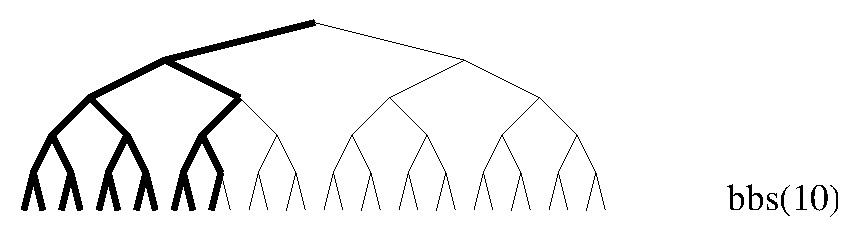
\includegraphics{bbs.eps}}
\end{center}
\caption{Bounded-backtrack search}
\label{figbbs}
\end{figure}
The {\em bbs} option of the search/6 predicate implements this:
\begin{quote}\begin{verbatim}
?-  queens(8, Xs),
    search(Xs, 0, input_order, indomain, bbs(20), []),
    writeln(Xs),
    fail.
[1, 5, 8, 6, 3, 7, 2, 4]
[1, 6, 8, 3, 7, 4, 2, 5]
[1, 7, 4, 6, 8, 2, 5, 3]
[1, 7, 5, 8, 2, 4, 6, 3]
No.
\end{verbatim}\end{quote}
Only the first 4 solutions are found, the next solution would have
required more backtracks than were allowed. 
Note that the solutions that are found are all located on the left hand
side of the search tree. This often makes sense because with a good
search heuristic, the solutions tend to be towards the left hand side.
Figure \ref{figbbs} illustrates the effect of bbs (note that the diagram
does not correspond to the queens example, it shows an unconstrained search
tree with 5 binary variables).


% - - - - - - - - - - - - - - - - - - - - - - - - - - - - - - - - - - -
\subsection{Depth Bounded Search}
\index{depth-bounded search} 
% - - - - - - - - - - - - - - - - - - - - - - - - - - - - - - - - - - -

A simple method of limiting search is to limit the depth of the search
tree. In many constraint problems with a fixed number of variables
this is not very useful, since all solutions occur at the same depth
of the tree. However, one may want to explore the tree completely
up to a certain depth and switch to an incomplete search method below this
depth. The search/6 predicate allows for instance the combination of
depth-bounded search with bounded-backtrack search. The following
explores the first 2 levels of the search tree completely, and does not
allow any backtracking below this level.
\begin{figure}
\begin{center}
\resizebox{0.6\textwidth}{!}{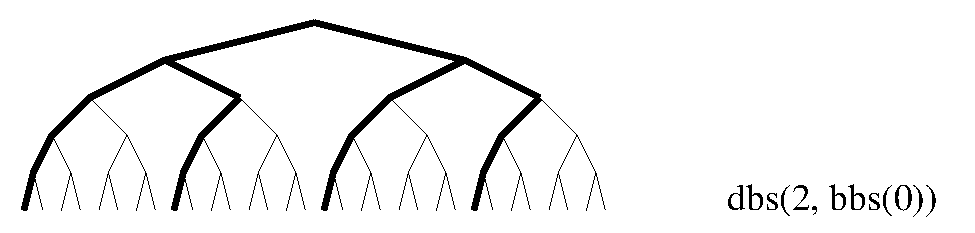
\includegraphics{dbsbbs.eps}}
\end{center}
\caption{Depth-bounded, combined with bounded-backtrack search}
\label{figdbsbbs}
\end{figure}
This gives 16 solutions, equally distributed over the search tree:
\begin{quote}\begin{verbatim}
?-  queens(8, Xs),
    search(Xs, 0, input_order, indomain, dbs(2,bbs(0)), []),
    writeln(Xs),
    fail.
[3, 5, 2, 8, 1, 7, 4, 6]
[3, 6, 2, 5, 8, 1, 7, 4]
[4, 2, 5, 8, 6, 1, 3, 7]
[4, 7, 1, 8, 5, 2, 6, 3]
[4, 8, 1, 3, 6, 2, 7, 5]
[5, 1, 4, 6, 8, 2, 7, 3]
[5, 2, 4, 6, 8, 3, 1, 7]
[5, 3, 1, 6, 8, 2, 4, 7]
[5, 7, 1, 3, 8, 6, 4, 2]
[6, 4, 1, 5, 8, 2, 7, 3]
[7, 1, 3, 8, 6, 4, 2, 5]
[7, 2, 4, 1, 8, 5, 3, 6]
[7, 3, 1, 6, 8, 5, 2, 4]
[8, 2, 4, 1, 7, 5, 3, 6]
[8, 3, 1, 6, 2, 5, 7, 4]
[8, 4, 1, 3, 6, 2, 7, 5]
No (0.18s cpu)
\end{verbatim}\end{quote}


% - - - - - - - - - - - - - - - - - - - - - - - - - - - - - - - - - - -
\subsection{Credit Search}
\index{credit search}
% - - - - - - - - - - - - - - - - - - - - - - - - - - - - - - - - - - -

Credit search\cite{beldiceanu:credit}
is a tree search method where the number of
nondeterministic choices is limited a priori.  This is achieved by
starting the search at the tree root with a certain integral amount of
credit.  This credit is split between the child nodes, their credit
between their child nodes, and so on.  A single unit of credit cannot
be split any further: subtrees provided with only a single credit unit
are not allowed any nondeterministics choices, only one path though these
subtrees can be explored, i.e. only one leaf in the subtree can be visited.
Subtrees for which no credit is left are pruned,
i.e.\ not visited.

The following code (a replacement for labeling/1)
implements credit search. For ease of understanding, it is
limited to boolean variables:
\begin{code}
% Credit search (for boolean variables only)
credit_search(Credit, Xs) :-
        (
            foreach(X, Xs),
            fromto(Credit, ParentCredit, ChildCredit, _)
        do
            ( var(X) ->
                ParentCredit > 0,  % possibly cut-off search here
                ( % Choice
                    X = 0, ChildCredit is (ParentCredit+1)//2
                ;
                    X = 1, ChildCredit is ParentCredit//2
                )
            ;
                ChildCredit = ParentCredit
            )
        ).
\end{code}
Note that the leftmost alternative (here X=0)
gets slightly more credit than the rightmost one (here X=1)
by rounding the child node's credit up rather than down. 
This is especially relevant when the leftover credit is down to 1:
from then on, only the leftmost alternatives will be taken until a
leaf of the search tree is reached. The leftmost alternative should
therefore be the one favoured by the search heuristics.

What is a reasonable amount of credit to give to a search?
In an unconstrained search tree, the credit is equivalent to the
number of leaf nodes that will be reached.
The number of leaf nodes grows exponentially with the number of
labelled variables, while tractable computations should have
polynomial runtimes. A good rule of thumb could therefore be to
use as credit the number of variables squared or cubed, thus enforcing
polynomial runtime.

Note that this method in its pure form allows choices only close to the
root of the search tree, and disallows choices completely below a certain
tree depth. This is too restrictive when the value selection strategy
is not good enough. A possible remedy is to combine credit search with
bounded backtrack search.


The implementation of credit search in the search/6 predicate works for
arbitrary domain variables: Credit is distributed by giving half to the
leftmost child node, half of the remaining credit to the second child node
and so on. Any remaining credit after the last child node is lost.
\begin{figure}
\begin{center}
\resizebox{0.6\textwidth}{!}{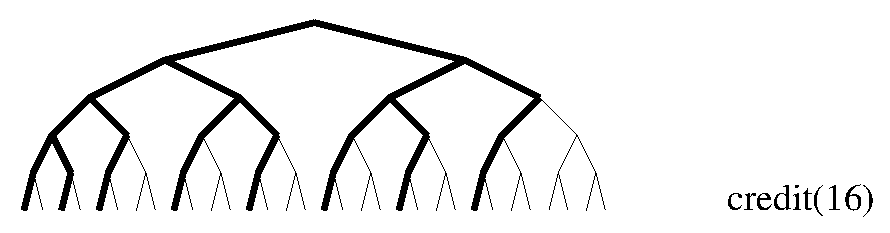
\includegraphics{credit.eps}}
\end{center}
\caption{Credit-based incomplete search}
\label{figcredit}
\end{figure}
In this implementation, credit search is always combined with another
search method which is to be used when the credit runs out.

When we use credit search in the queens example, we get a limited number
of solutions, but these solutions are not the leftmost ones (like with
bounded-backtrack search), they are
from different parts of the search tree, although biased towards the left:
\begin{quote}\begin{verbatim}
?- queens(8, Xs),
   search(Xs, 0, input_order, indomain, credit(20,bbs(0)), []),
   writeln(Xs),
   fail.
[2, 4, 6, 8, 3, 1, 7, 5]
[2, 6, 1, 7, 4, 8, 3, 5]
[3, 5, 2, 8, 1, 7, 4, 6]
[5, 1, 4, 6, 8, 2, 7, 3]
No.
\end{verbatim}\end{quote}
We have used a credit limit of 20. When credit runs out, we switch to
bounded backtrack search with a limit of 0 backtracks.



% - - - - - - - - - - - - - - - - - - - - - - - - - - - - - - - - - - -
\subsection{Timeout}
\index{timeout}
% - - - - - - - - - - - - - - - - - - - - - - - - - - - - - - - - - - -

Another form of incomplete tree search is simply to use time-outs.
\index{bb_min/3}
\index{bb_min/6}
The branch-and-bound primitives {\tt bb_min/3,6} allow
a maximal runtime to be specified. If a timeout occurs, the best solution
found so far is returned instead of the proven optimum.

A general timeout is available from the library {\tt test_util}.
It has parameters {\tt timeout(Goal, Seconds, TimeOutGoal)}.
When {\tt Goal} has run for
more than {\tt Seconds} seconds, it is aborted and {\tt TimeOutGoal}
is called instead. 

%----------------------------------------------------------------------
\subsection{Limited Discrepancy Search}
\index{limited discrepancy search}
%----------------------------------------------------------------------

% - - - - - - - - - - - - - - - - - - - - - - - - - - - - - - - - - - -
%\subsubsection{Introduction}
% - - - - - - - - - - - - - - - - - - - - - - - - - - - - - - - - - - -

Limited discrepancy search ({\em LDS}) is a search method that assumes
the user has a good heuristic for directing the search.  A perfect
heuristic would, of course, not require any search.  However most
heuristics are occasionally misleading.  Limited Discrepancy Search
follows the heuristic on almost every decision.  The
``discrepancy'' is a measure of the degree to which it fails to follow
the heuristic.  LDS starts searching with a discrepancy of $0$ (which
means it follows the heuristic exactly).  Each time LDS fails to find
a solution with a given discrepancy, the discrepancy is increased and
search restarts.  In theory the search is complete, as eventually the
discrepancy will become large enough to admit a solution, or cover
the whole search space.  In practice, however, it is only beneficial
to apply LDS with small discrepancies.  Subsequently, if no solution
is found, other search methods should be tried.
The definitive reference to LDS is \cite{harvey95:lds:inp}
%\begin{quote}
%Limited Discrepancy Search, Harvey and Ginsberg,
%pp.607-613, Proc. IJCAI'95
%\end{quote}

\index{discrepancy}
There are different possible ways of measuring discrepancies.
The one implemented in the search/6 predicate is a variant of the
original proposal. It considers the first
value selection choice as the heuristically best value with
discrepancy 0, the first alternative has a discrepancy of 1, the
second a discrepancy of 2 and so on.
\begin{figure}
\begin{center}
\resizebox{0.6\textwidth}{!}{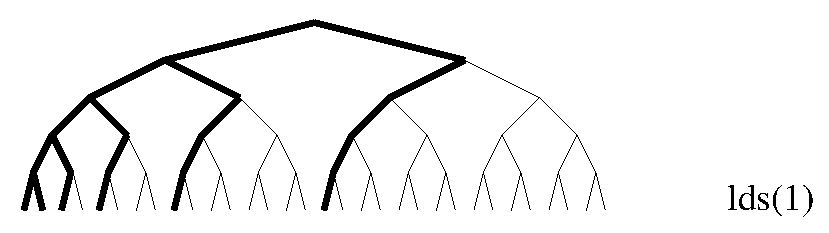
\includegraphics{lds.eps}}
\end{center}
\caption{Incomplete search with LDS}
\label{figlds}
\end{figure}

As LDS relies on a good heuristic, it only makes sense for the queens
problem if we use a good heuristic, e.g. first-fail variable selection
and indomain-middle value selection. Allowing a discrepancy of 1 yields
4 solutions:
\begin{quote}\begin{verbatim}
?- queens(8, Xs), 
   search(Xs, 0, first_fail, indomain_middle, lds(1), []),
   writeln(Xs),
   fail.
[4, 6, 1, 5, 2, 8, 3, 7]
[4, 6, 8, 3, 1, 7, 5, 2]
[4, 2, 7, 5, 1, 8, 6, 3]
[5, 3, 1, 6, 8, 2, 4, 7]
No.
\end{verbatim}\end{quote}

The reference also suggests that combining LDS with Bounded Backtrack
Search ({\em BBS}) yields good behaviour. The search/6 predicate
accordingly supports the combination of LDS with BBS and DBS.
The rationale for this is that heuristic choices typically get
more reliable deeper down in the search tree.


%% - - - - - - - - - - - - - - - - - - - - - - - - - - - - - - - - - - -
%\subsubsection{Limited Discrepancy Search using a Static Heuristic}
%% - - - - - - - - - - - - - - - - - - - - - - - - - - - - - - - - - - -
%
%We start by assuming a static heuristic, which is a complete
%assignment to the problem variables specified in advance of the
%search.  The predicate supporting static LDS takes a list of variables
%(those which are to be labelled) and a list of values (one heuristic
%value for each variable, respectively).  Each variable has a finite
%domain, and its heuristic value should belong to its domain (though
%the LDS search can still succeed even if this is not the case).
%
%The measure of discrepancy, in this case, is simply the number of
%variables labelled differently to the heuristic.  Thus the maximum
%discrepancy is just the number of variables to be
%labelled.
%
%LDS search is implemented in the file
%{\tt lds.ecl} in the {\tt doc/examples} directory of your
%{\eclipse} installation. You can copy this file and load it with
%\begin{quote}\begin{alltt}
%:- use_module(lds).
%\end{alltt}\end{quote}
%Static LDS search is then available via the predicate
%{\bf static_lds(Var, Vals, Discrepancy)} whose arguments are
%\begin{description}
%\item[Vars] the list of problem variables.  Some of the
%variables may already be instantiated.  The others
%must have associated finite domains.
%\item[Vals] the list of values according to the heuristic.  It
%must be the same length as Vars, and the heuristic
%must match the value, in case the variable is
%already instantiated.
%\item[Discrepancy] the discrepancy of the solution returned.  Typically this
%is an output of the search (an integer between $0$ and the number of
%variables), but it can also be used as an input.
%\end{description}
%The finite domain library must be loaded, and the variables must have
%finite domains.  An example invocation is:
%\begin{quote}\begin{alltt}
%?- [X,Y,Z]::1..3, X+Y+Z#=5, static_lds([X,Y,Z],[1,2,3],D).
%\end{alltt}\end{quote}
%The answers are returned on backtracking in the following order:
%\begin{itemize}
%\item
%X = 1
%Y = 2
%Z = 2
%D = 1     
%\item
%X = 1
%Y = 1
%Z = 3
%D = 1     
%\item
%X = 1
%Y = 3
%Z = 1
%D = 2     
%\item
%X = 2
%Y = 2
%Z = 1
%D = 2     
%\item
%X = 2
%Y = 1
%Z = 2
%D = 3     
%\item
%X = 3
%Y = 1
%Z = 1
%D = 3
%\end{itemize}
%
%
%% - - - - - - - - - - - - - - - - - - - - - - - - - - - - - - - - - - -
%\subsubsection{Limited Discrepancy Search using a Dynamic Heuristic}
%% - - - - - - - - - - - - - - - - - - - - - - - - - - - - - - - - - - -
%
%Often the heuristic value is calculated on the fly, during search.  To
%cope with this we use the {\eclipse} ``tentative value'' facility in
%{\eclipse}'s {\em repair} library. 
%The heuristic is stored with the variable as its tentative value. 
%
%The tentative value may be changed during search.  For example if a
%variable is instantiated as a consequence of constraint propagation
%during search, its tentative value is automatically changed to its
%actual value. 
%
%Dynamic LDS search is available in {\eclipse} via the predicate
%{\bf dynamic_lds(Vars, Discrepancy)}.
%Each variable in the list of variables {\em Vars} 
%must have a tentative value.
%
%An example invocation is:
%\begin{quote}\begin{alltt}
%?- [X,Y,Z]::1..3, [X,Y,Z] tent_set [1,2,3], X+Y+Z#=5,
%   dynamic_lds([X,Y,Z],D).
%\end{alltt}\end{quote}
%The answers are returned on backtracking in the following order.
%Notice that the first solution has a discrepancy of $0$, because
%constraint propagation instantiates the third variable to $2$,
%thus changing its tentative value from $3$ to $2$.
%\begin{itemize}
%\item
%X = 1
%Y = 2
%Z = 2
%D = 0    
%\item
%X = 1
%Y = 1
%Z = 3
%D = 1    
%\item
%X = 1
%Y = 3
%Z = 1
%D = 1    
%\item
%X = 2
%Y = 2
%Z = 1
%D = 1    
%\item
%X = 3
%Y = 1
%Z = 1
%D = 1    
%\item
%X = 2
%Y = 1
%Z = 2
%D = 2 
%\end{itemize}
%
%% - - - - - - - - - - - - - - - - - - - - - - - - - - - - - - - - - - -
%\subsubsection{LDS and BBS Combined}
%% - - - - - - - - - - - - - - - - - - - - - - - - - - - - - - - - - - -
%
%The two search techniques, BBS and LDS, can be merged quite simply in
%{\eclipse}, so that for each discrepancy level only a limited number of
%backtracks are allowed.  
%
%An example invocation is:
%\begin{quote}\begin{alltt}
%?- Vars=[X,Y,Z], Vars::1..3, Vars tent_set [1,2,3], X+Y+Z#=6,
%   bbs_dynamic_lds(Vars,4,D).
%\end{alltt}\end{quote}
%The answers are returned on backtracking in the following order:
%\begin{itemize}
%\item
%X = 1
%Y = 2
%Z = 3
%D = 0   
%\item
%X = 1
%Y = 3
%Z = 2
%D = 1   
%\item
%X = 2
%Y = 2
%Z = 2
%D = 1   
%\item
%X = 3
%Y = 2
%Z = 1
%D = 1   \\
%Backtrack limit exceeded
%\item
%X = 2
%Y = 1
%Z = 3
%D = 2 \\
%Backtrack limit exceeded
%\end{itemize}

%----------------------------------------------------------------------
\section{Exercises}
%----------------------------------------------------------------------

For exercises 1-3, start from the constraint model for the queens problem
given in section \ref{queenscode}. It is available in the examples directory
as queens_ic.ecl.

\begin{enumerate}

\item Use the search/6 predicate from the ic_search library and the
standard model for the queens problem (given below) to find ONE
solution to the 42-queens problem.
With a naive search strategy this requires millions of backtracks.
Using heuristics and/or incomplete search, try to find a solution
in less than 100 backtracks!


\item How many solutions does the 9-queens problem have?


\item Solve the "8 sticky queens problem": Assume that the queens
in neighbouring columns want to stick together as close as possible.
Minimize the sum of the vertical distances between neighbouring queens.
What is the best and what is the worst solution for this problem?


\item For given N, create a list of length N whose members are numbers
between 1 and N (inclusive), which are all different (easy so far) 
and satisfy the following constraint.
For each element E of the list, its successors are divided into two sets,
   \begin{itemize}
   \item BiggerE: the successors which are greater than E and
   \item SmallerE: the successors less than E.
   \end{itemize}
(Thus no successor takes the same value as E).
The cardinalities of the sets BiggerE and SmallerE differ by at most 1. 


\item A harder version of the problem is similar.
For given N, create a list of length N whose members are numbers
between 1 and some upper bound Max (start with, say Max = $N^2$), 
which are all different (easy so far) 
and satisfy the following (more complex) constraint.
For each K from 1..N, call the Kth element of the list Ek. 
Its successors are divided into two sets, as before:
   \begin{itemize}
   \item BiggerEk: the successors which are greater than or equal to Ek + K and
   \item SmallerEk: the successors less than or equal to Ek - K.
   \end{itemize}
(Thus no successor takes a value between Ek-K+1 and Ek+K-1.)
The cardinalities of the sets BiggerEk and SmallerEk differ 
by at most 1. 

What is the smallest upper bound Max for which there is a feasible solution?

\end{enumerate}

%HEVEA\cutend
